%! Author = Wiktor Rostkowski
%! Date = 13/06/2024

\chapter{Prezentacja systemu}
\label{ch:prezentacja-systemu}



\section{Widok głównej stron}
\label{sec:mapawidok}

Aplikacja prezentuje użytkownikom interaktywną mapę z zaznaczonymi atrakcjami turystycznymi (POI). 
Na głównym ekranie znajdują się różne elementy interfejsu, które ułatwiają nawigację i dostęp do kluczowych funkcji.

Główną część widoku aplikacji stanowi interaktywna mapa, na której zaznaczone są punkty zainteresowania. Użytkownicy mogą:
\begin{itemize}
 \item   Kliknąć na poszczególne POI, aby uzyskać więcej informacji o danej atrakcji.
 \item   Zaznaczać i dodawać POI do koszyka.
 \item  Korzystać z opcji wyznaczania tras pomiędzy wybranymi punktami.
\end{itemize}
Mapa jest interaktywna i responsywna, pozwalając użytkownikom na swobodne powiększanie, pomniejszanie oraz przesuwanie widoku w celu znalezienia interesujących miejsc.

\begin{figure}[H]
    \centering
    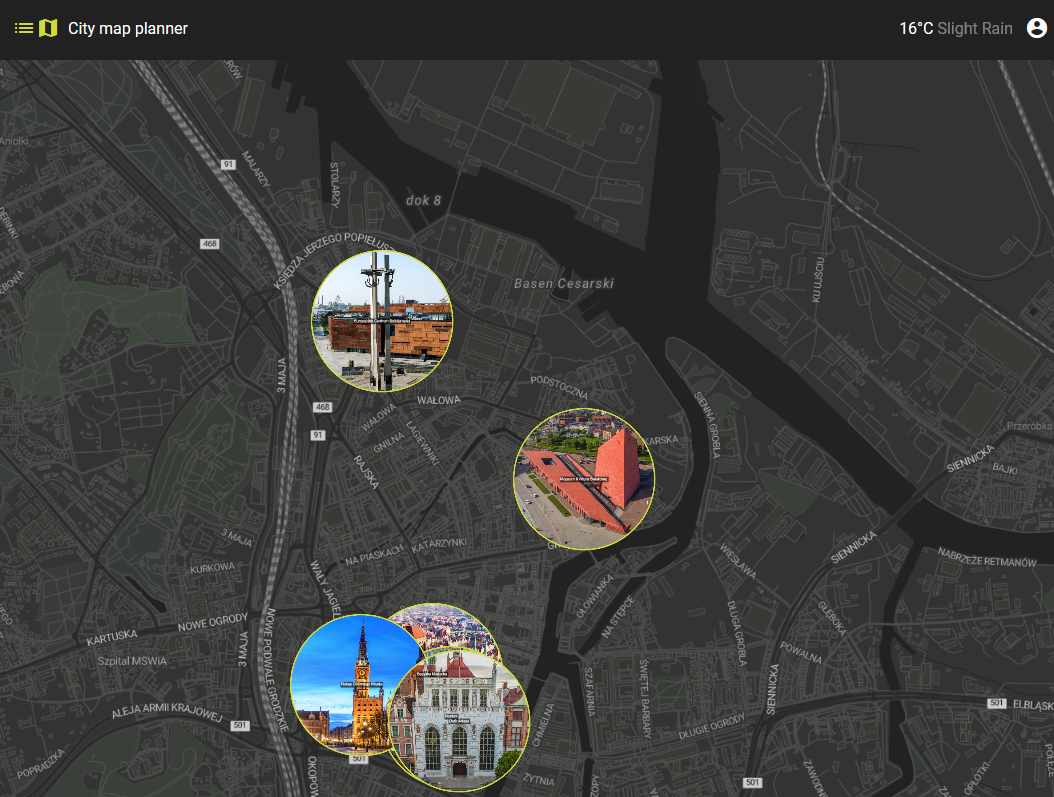
\includegraphics[width=1\textwidth]{attachments/mapawidok}
    \caption{Widok głównej strony}
    \label{fig:mapawidok}
    \end{figure}
    \begin{figure}[H]
        \centering
        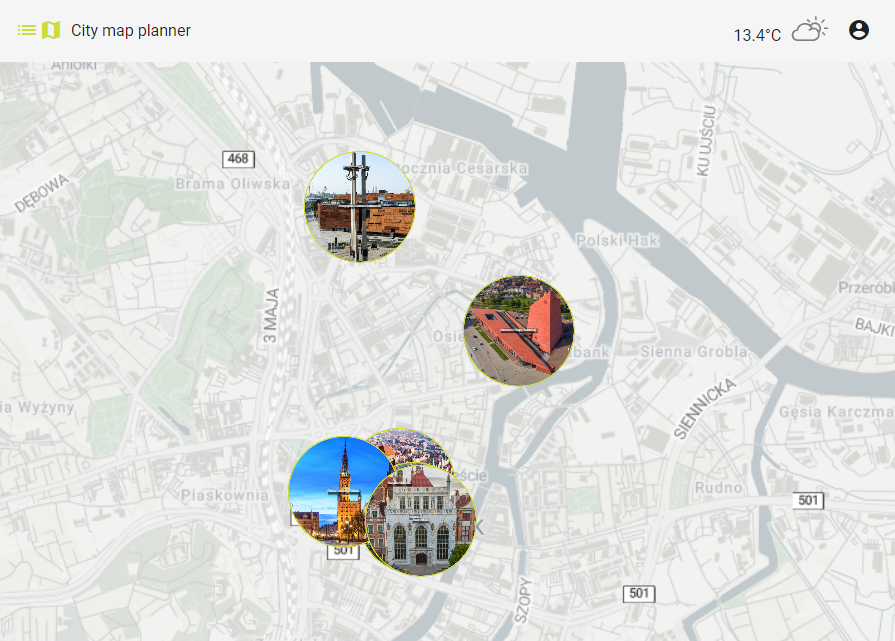
\includegraphics[width=1\textwidth]{attachments/mapawidok-light}
        \caption{Widok głównej strony wersja jasna}
        \label{fig:mapawidok}
        \end{figure}
        \begin{figure}[H]
            \centering
            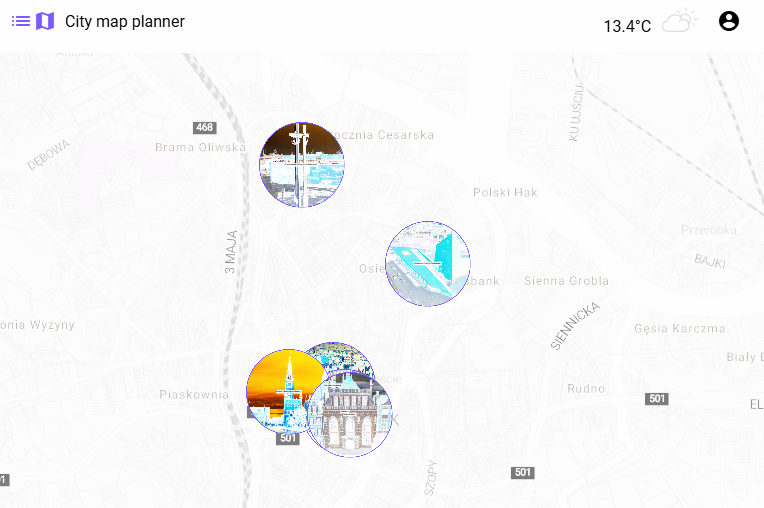
\includegraphics[width=1\textwidth]{attachments/mapawidok-high-contrast}
            \caption{Widok głównej strony wersja wysoki kontrast}
            \label{fig:mapawidok}
            \end{figure}

\subsection{Pasek Nawigacji}
\label{sec:pasek-nawigacji}
Pasek główny z nawigacją znajduje się na górze ekranu, zapewniając szybki dostęp do najważniejszych sekcji aplikacji. Na pasku znajdują się następujące elementy:
\begin{itemize}
    \item link do listy POI;
    \item link do strony głównej;
    \item aktualna Temperatura;
    \item obok temperatury wyświetlana jest ikona pogody(np. deszcz, słońce), która wizualnie przedstawia obecne warunki atmosferyczne;
    \item jeśli użytkownik wybrał jakieś punkty zainteresowania, pojawia się link do koszyka;
    \item link do zarządzania konta użytkownika;
\end{itemize}
\begin{figure}[H]
    \centering
    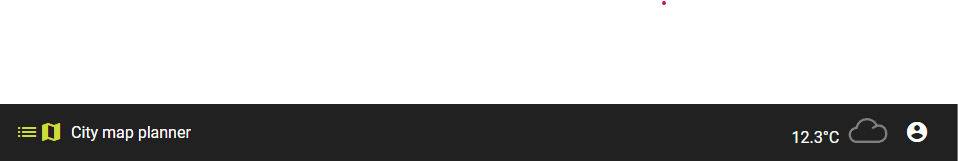
\includegraphics[width=1\textwidth]{attachments/nav-baner}
    \caption{Pasek Nawigacji}
    \label{fig:pasek-nawigacji}
\end{figure}

\section{Widok pojedynczej atrakcji}
\label{sec:atrakcjawidok}
Widok pojedynczej atrakcji w aplikacji został zaprojektowany tak, aby dostarczyć 
użytkownikom wszystkie niezbędne informacje w przejrzysty i estetyczny sposób. 
Składa się z kilku kluczowych elementów, które pomagają użytkownikowi zapoznać się z daną atrakcją oraz podjąć decyzję o jej odwiedzeniu.
\newline
Zdjęcie atrakcji:
Na samej górze ekranu znajduje się duże, wysokiej jakości zdjęcie atrakcji. 
Zdjęcie to pozwala użytkownikom wizualnie ocenić miejsce i zyskać wstępne wrażenie. Jest to pierwsza rzecz, którą widzą użytkownicy, co ma na celu przyciągnięcie ich uwagi i zainteresowanie.
\newline
Tytuł atrakcji:
Bezpośrednio pod zdjęciem znajduje się tytuł atrakcji. Jest to nazwa miejsca, która jest 
wyraźnie wyeksponowana dużą czcionką, aby użytkownik od razu wiedział, o jakiej atrakcji mowa.
\newline
Opis atrakcji:
Pod tytułem znajduje się szczegółowy opis atrakcji. 
Opis zawiera informacje na temat historii, znaczenia, dostępnych aktywności oraz innych interesujących faktów, które mogą 
zainteresować użytkownika. Tekst jest sformatowany w sposób przejrzysty, z podziałem na akapity, aby ułatwić czytanie.
\newline
Rekomendowana pogoda:
Na samym dole widoku znajduje się sekcja dotycząca rekomendowanej 
pogody do odwiedzenia atrakcji. Sekcja ta zawiera ikony pogody (np. słońce, chmury, deszcz). 
Informacje te pomagają użytkownikom zaplanować wizytę w najlepszym możliwym czasie.
\newline
Aplikacja została wykonana z możliwością wyboru dwóch motywów: ciemnego i jasnego. 
Użytkownicy mogą dostosować wygląd interfejsu do swoich preferencji oraz warunków oświetleniowych, co zwiększa komfort użytkowania aplikacji.

\begin{figure}[H]
        \centering
        \includegraphics[width=1\textwidth]{attachments/atrakcjawidok}
        \caption{Widok pojedynczej atrakcji}
        \label{fig:mapawidok}
\end{figure}
\begin{figure}[H]
    \centering
    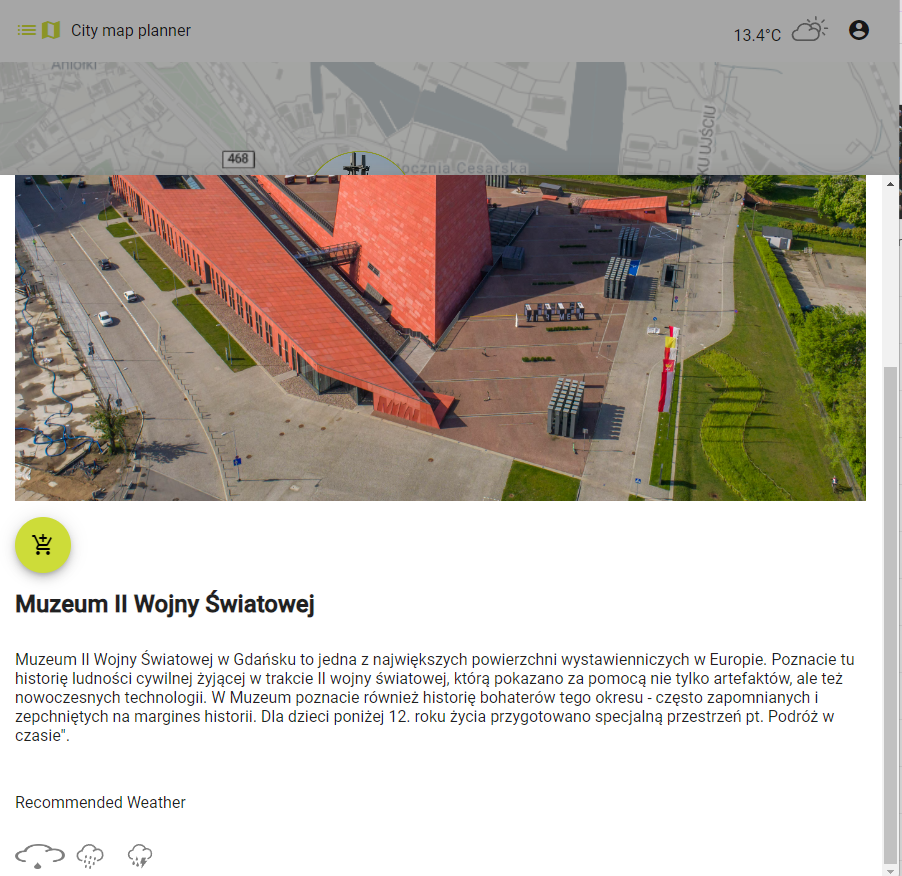
\includegraphics[width=1\textwidth]{attachments/atrakcjawidok-light}
    \caption{Widok pojedynczej atrakcji}
    \label{fig:mapawidok}
\end{figure}
\section{Widok koszyka}
\label{sec:koszyk}

Moduł koszyk w aplikacji pełni funkcję przechowywania i zarządzania wybranymi punktami zainteresowania (POI). 
Zaprojektowany z myślą o wygodzie użytkownika, widok koszyka umożliwia łatwe przeglądanie, modyfikowanie oraz usuwanie dodanych POI.

    \begin{figure}[H]
        \centering
        \includegraphics[width=1\textwidth]{attachments/koszyk}
        \caption{Widok koszyka}
        \label{fig:koszyk}
\end{figure}

\section{Widok kalendarza}
\label{sec:atrakcjawidok}



\begin{figure}[H]
        \centering
        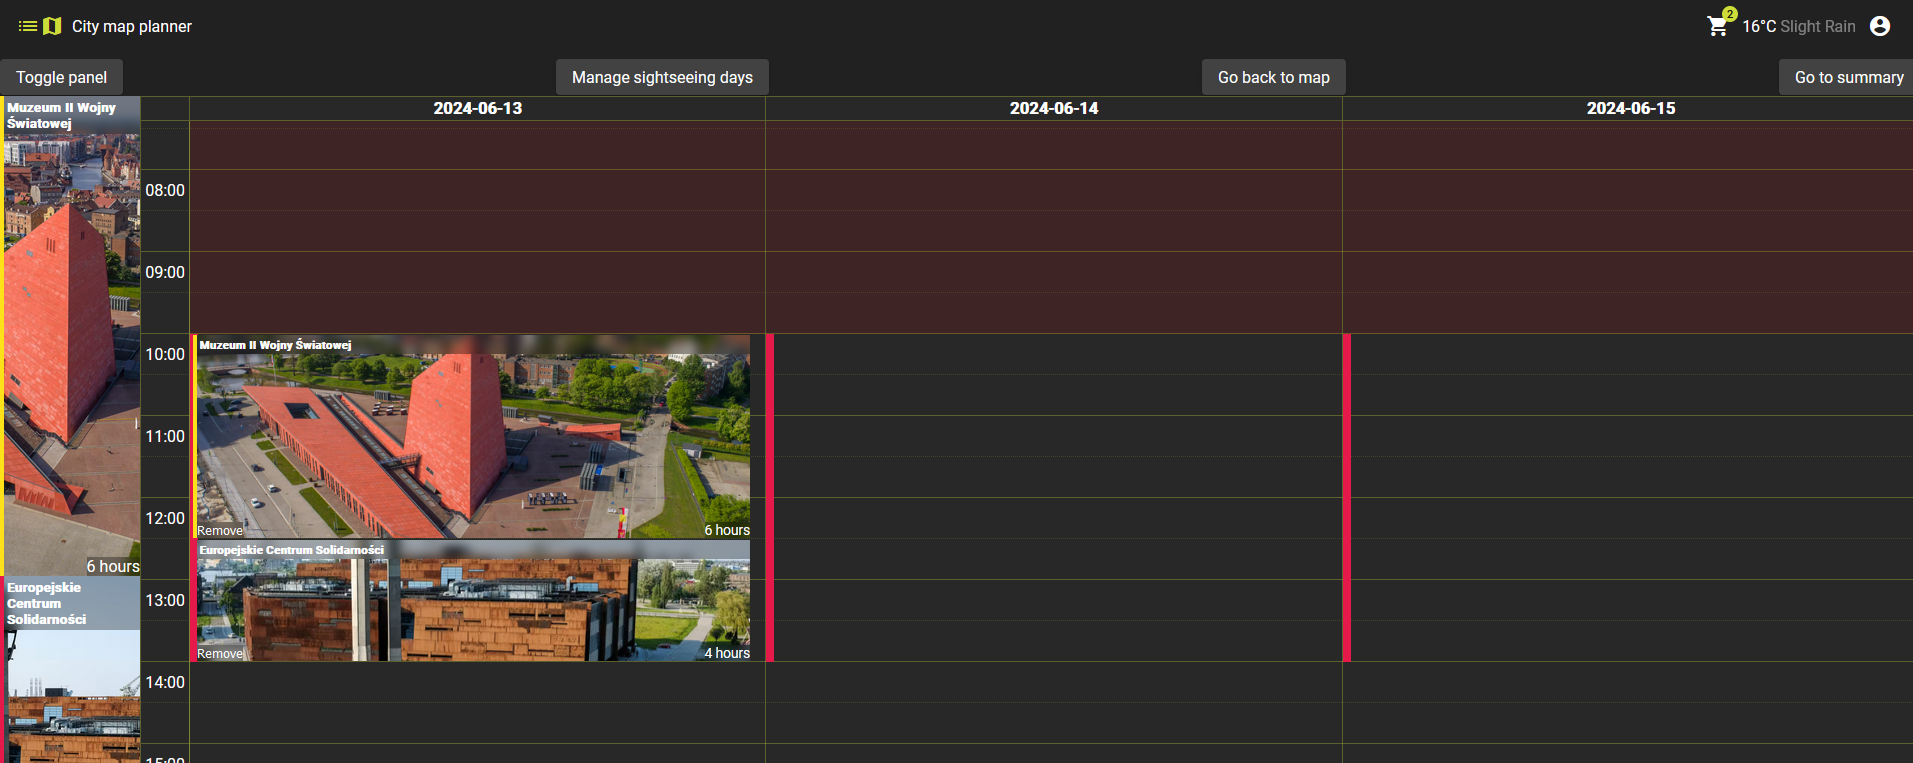
\includegraphics[width=1\textwidth]{attachments/kalendarz}
        \caption{Widok kalendarza}
        \label{fig:kalendarz}
\end{figure}
\begin{figure}[H]
    \centering
    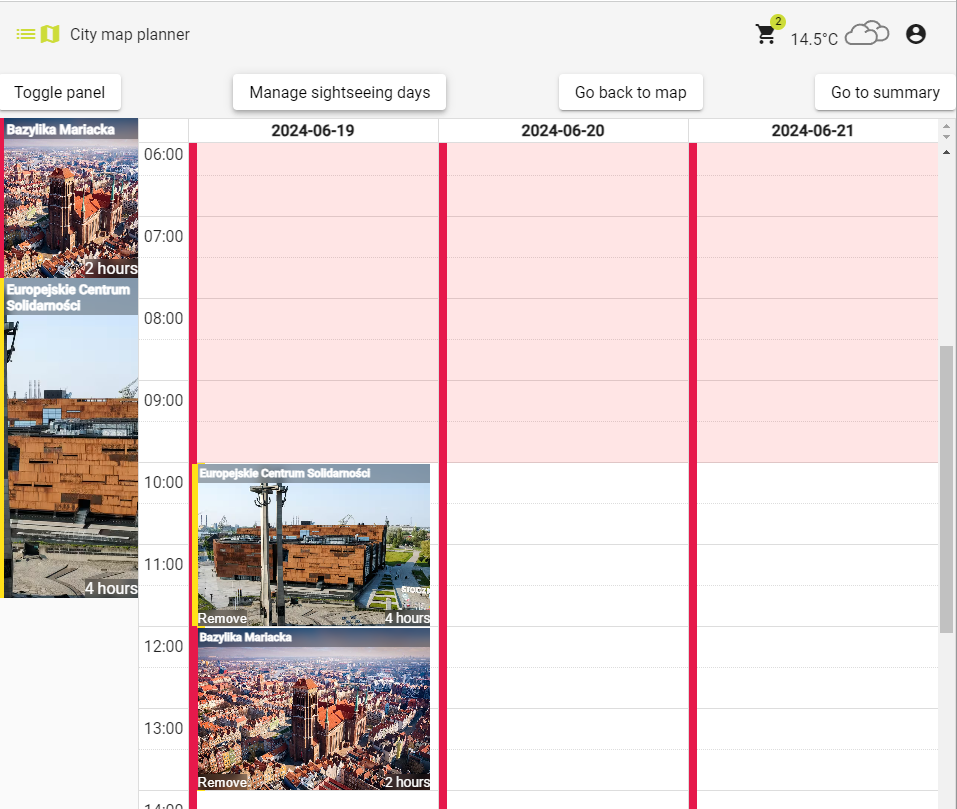
\includegraphics[width=1\textwidth]{attachments/kalendarz-light}
    \caption{Widok kalendarza jasny}
    \label{fig:kalendarz-light}
\end{figure}
\section{Widok podsumowania}
\label{sec:atrakcjawidok}
\begin{figure}[H]
    \centering
    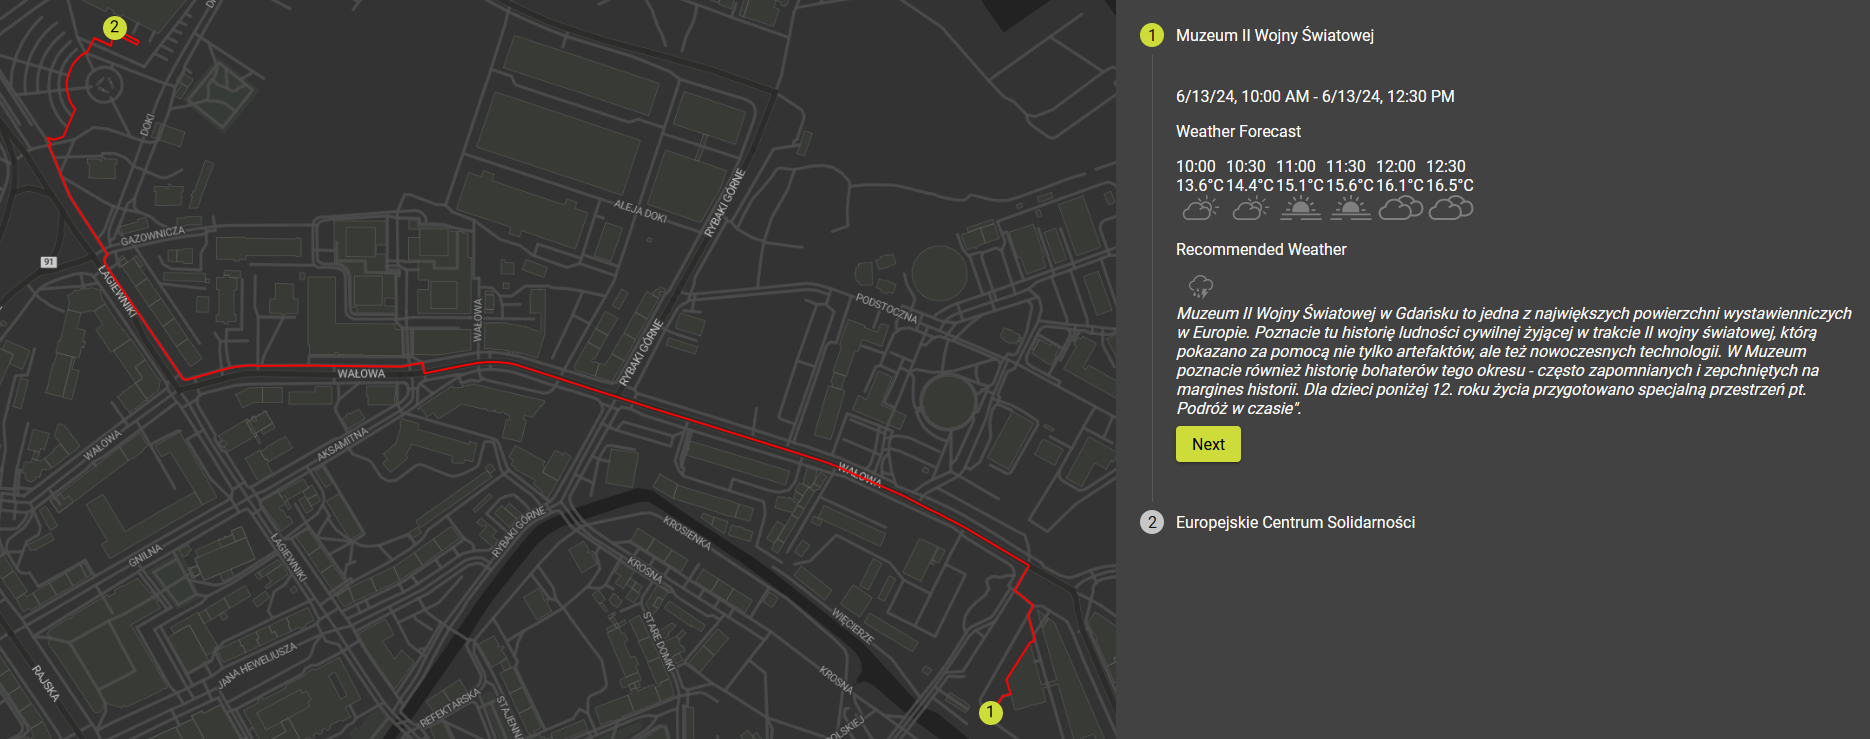
\includegraphics[width=1\textwidth]{attachments/podsumowanie}
    \caption{Widok podsumowanie}
    \label{fig:podsumowanie}
\end{figure}
\begin{figure}[H]
    \centering
    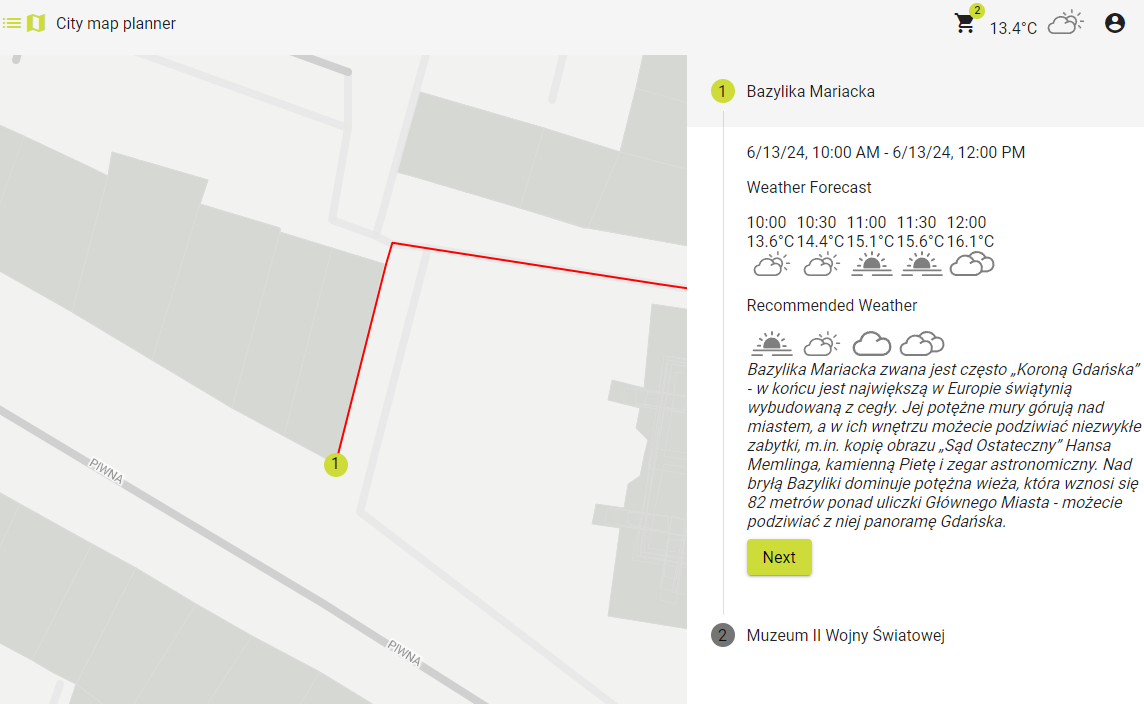
\includegraphics[width=1\textwidth]{attachments/podsumowanie-light}
    \caption{Widok podsumowanie wersja jasna}
    \label{fig:podsumowanie-light}
\end{figure}
\section{Widok Listy POI}
\label{sec:poilist}

\begin{figure}[H]
    \centering
    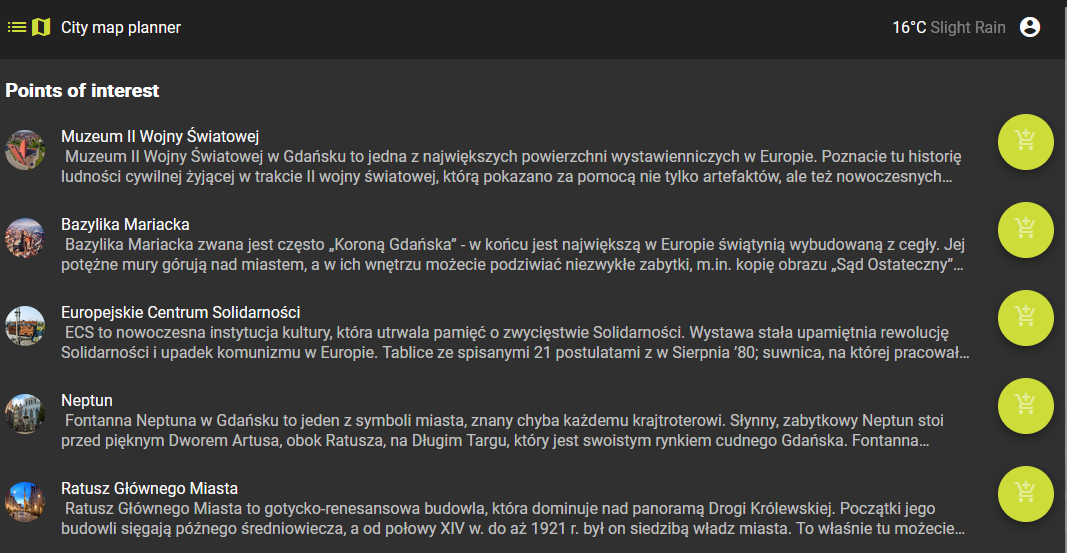
\includegraphics[width=1\textwidth]{attachments/poilist}
    \caption{Widok listy wszystkich dostępnych atrakcji}
    \label{fig:poilist}
\end{figure}


\section{Widok zarządzania kotem użytkownika}
\label{sec:user}

\begin{figure}[H]
    \centering
    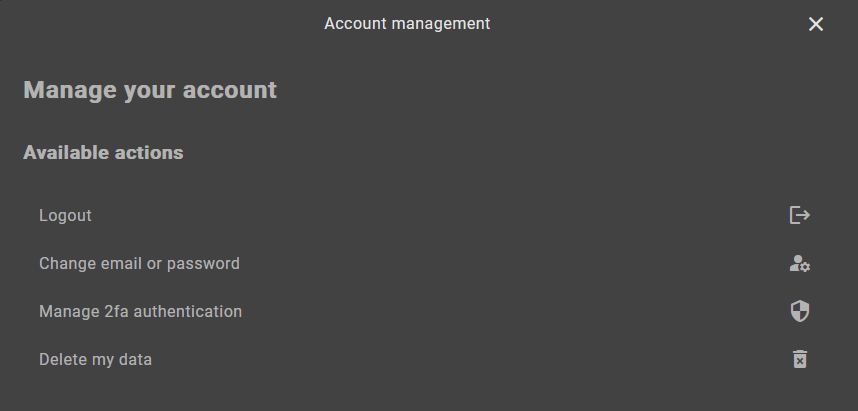
\includegraphics[width=1\textwidth]{attachments/user}
    \caption{Widok panelu zarządzania użytkownikiem}
    \label{fig:user}
\end{figure}

\section{Widok Logowania}
\label{sec:logowanie}

\begin{figure}[H]
    \centering
    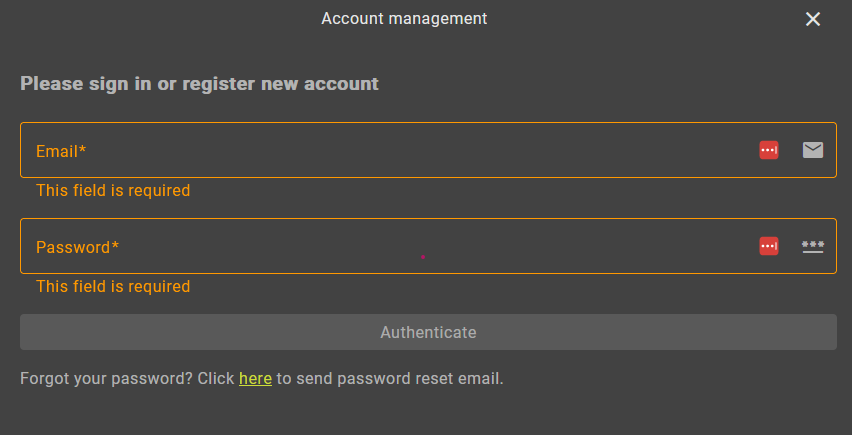
\includegraphics[width=1\textwidth]{attachments/logowanie}
    \caption{Widok panelu logowania}
    \label{fig:logowanie}
\end{figure}

\section{Widok zarządzania wszystkimi POI}
\label{sec:manage}

\begin{figure}[H]
    \centering
    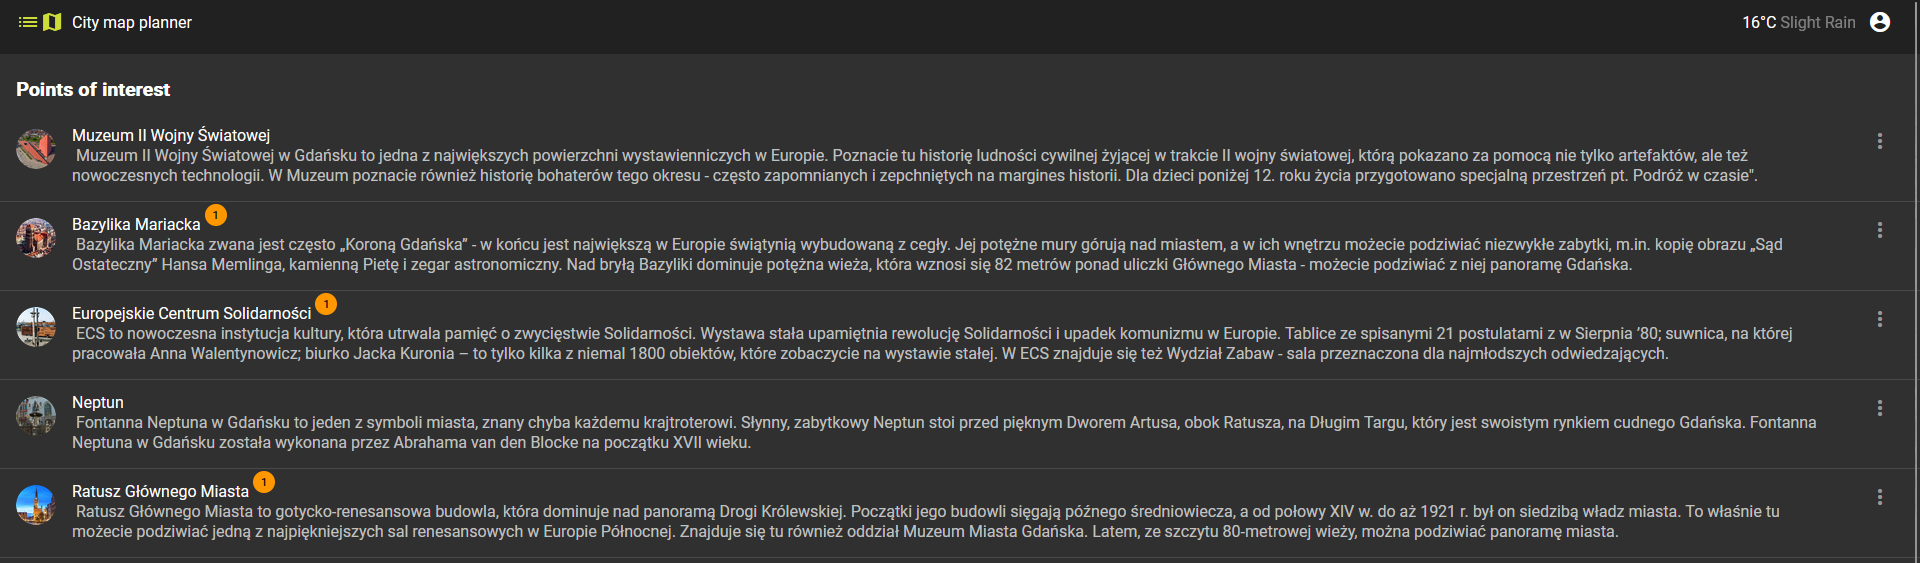
\includegraphics[width=1\textwidth]{attachments/poi-manage}
    \caption{Widok panelu zarządzania wszystkimi POI}
    \label{fig:poi-manage}
\end{figure}

\begin{figure}[H]
    \centering
    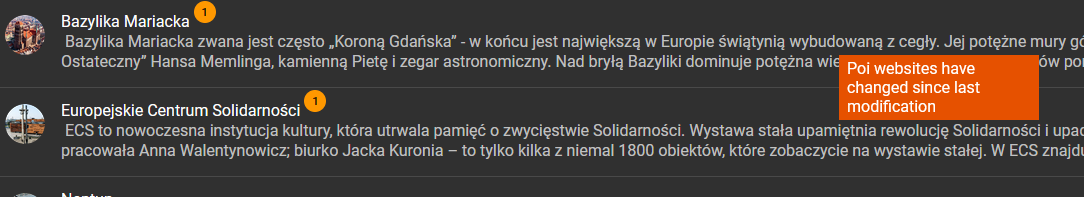
\includegraphics[width=1\textwidth]{attachments/poi-notify}
    \caption{Informacja o potrzebie sprawdzenia aktualności danych}
    \label{fig:ManageNofify}
\end{figure}

\begin{figure}[H]
    \centering
    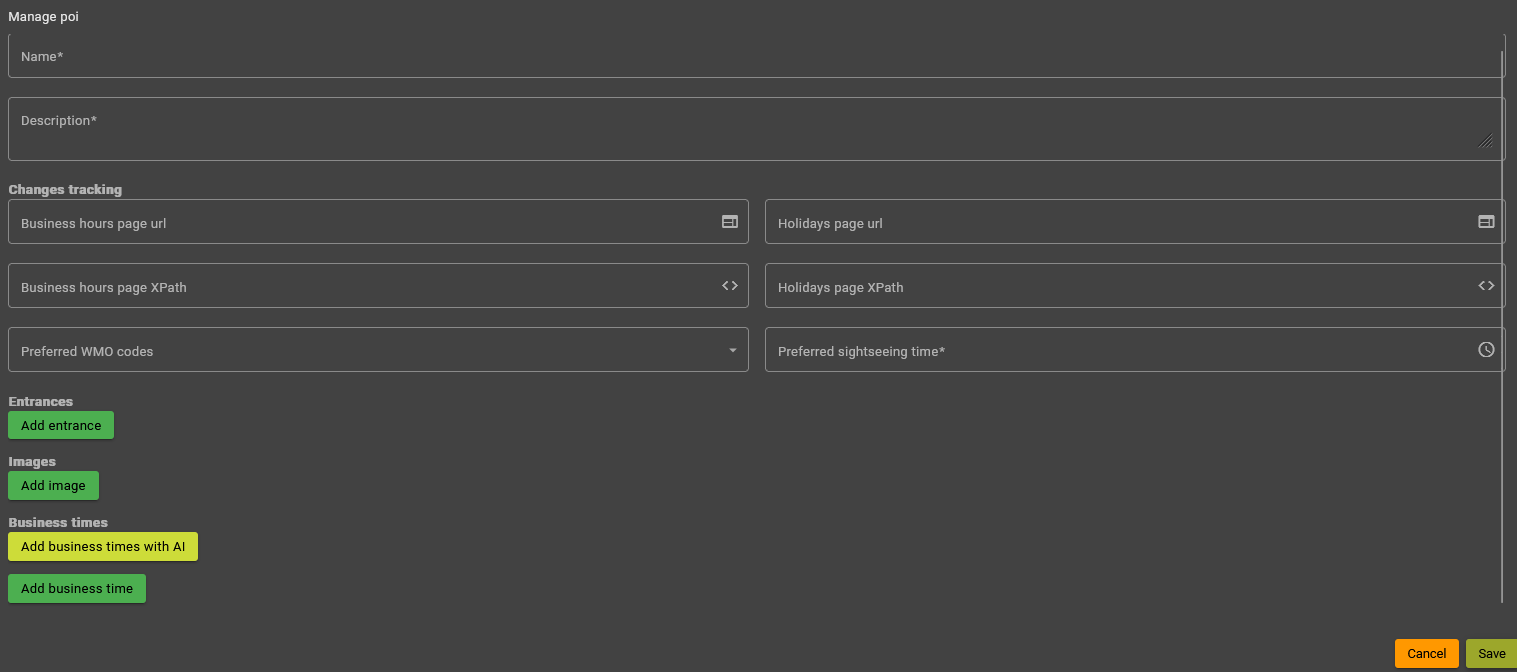
\includegraphics[width=1\textwidth]{attachments/addpoi}
    \caption{Widok panelu dodawania POI}
    \label{fig:ManageNofify}
\end{figure}